\chapter{Data}\label{chapter:data}
In this chapter we are going to introduce the two main text corpora used in this thesis. This includes an explanation of their content and how we preprocess it in order to obtain the datasets for training our models. A basic n-gram analysis of the corpora is also prepared in for later usage in the Chapter~\ref{analysis_of_results}.

\section{Datasets}
We are using two different datasets for the experiments. The first is the current version of the OpenSubtitles corpus \cite{Lison:2016} that contains subtitles from over $300,000$ movies. The second is a datasets containing all comments posted on the website Reddit\footnote{https://www.reddit.com/} from 2006 until 2015. Some general information can be found in table~\ref{data:raw:table}

\begin{table}[H]
	\centering
	\begin{adjustbox}{max width=\textwidth}
	  \begin{tabular}{llcccl}
	    \toprule
	    &  \specialcell{Short name}
	    &  \specialcell{Size\\(Gb)}
	    &  \specialcell{Lines\\(Million)}
	    &  \specialcell{Data format}
	    &  \specialcell{Source} \\
	    \midrule
	    OpenSubtitles 2016 & OpenSubtitles & 93  & 338 & XML & \cite{Lison:2016} \\
	    Reddit Submission Corpus  &Reddit &885  & 1'650 & JSON  &  Reddit Comments Corpus\protect\footnotemark\\
	    \bottomrule
	  \end{tabular}
	\end{adjustbox}
	\caption{Origin and some additional information about the raw corpora.}
	\label{data:raw:table}
\end{table}
\footnotetext{https://archive.org/details/2015\_reddit\_comments\_corpus}

The two datasets differ in several aspects: Since the OpenSubtitles corpus is extracted from subtitles of a large number of movies, it represents a corpora of \emph{spoken} language. In contrast, the Reddit dataset only consists of comments posted on the website and hence represents written, partially colloquial, language. These two type of language usually differ greatly in how they are used\footnote{A good comparison can be found on the website of the University of Westminister: http://www2.wmin.ac.uk/eic/learning-skills/literacy/sp\_vs\_writ\_dif.shtml}.

\section{Structure of the Raw Corpora}
\label{data:structure_of_corpora}
The following two paragraphs explain how the raw datasets are structured and how the raw utterances are extracted from them.

\paragraph{OpenSubtitles} The OpenSubtitles corpus is structured via XML files, each one containing all utterances from a single movie (see figure~\ref{data:opensubtitles:xml_example}). Each XML is structured the same way: It starts with the declaration of the \texttt{<document>} tag and an \texttt{id} attribute signifying which movie the subtitles are from. However, as our research has shown, the value of the \texttt{id} attribute cannot be used to decide whether subtitles of a certain movie have already been processed, because there are files with the same \texttt{id} but different content. After the \texttt{<document>} the actual utterances are listed in \texttt{<s>} tags. Each of these \texttt{<s>} contains multiple \texttt{<w>} tags that contain the actual words uttered in this utterance. Furthermore, one can see that there are also \texttt{<time>} tags that contains a timestamp when the utterance started and one when the utterance ended. These timestamps are later used for the time-lag analysis in the chapter~\ref{data:opensubtitles:time_lag_analysis}. There is absolutely no indication on turn-taking, which forces us handle each utterance as an utterance by a different person, even though it could certainly be uttered by the same.\\


\begin{figure}[thp]
	\centering
	\begin{tabular}{c}  % the tabular makes the listing as small as possible and centers it
		\begin{lstlisting}[language=XML]
		<?xml version="1.0" encoding="utf-8"?>
		<document id="4955664">
			<s id="1">
				<time id="T19S" value="00:01:54,300" />
				<w id="15.1">Here</w>
				<w id="15.2">it</w>
				<w id="15.3">'s</w>
				<w id="15.4">your</w>
				<w id="15.5">brain</w>
				<w id="15.6">versus</w>
				<w id="15.7">the</w>
				<w id="15.8">opponent</w>
				<w id="15.9">'s</w>
				<w id="15.10">.</w>
				<time id="T19E" value="00:01:58,250" />
			</s>
			...
		</document>
		\end{lstlisting}
	\end{tabular}
	\caption{Example XML entry from the OpenSubtitles corpus.}
	\label{data:opensubtitles:xml_example}
\end{figure}

\todo{opus aufbau png}

\paragraph{Reddit} The Reddit corpus is structured in huge plain text files for each year, where comments are available. In our case, the comments available are from ranging from 2006 up to the year 2015. For each year, there is a separate plain text file containing one JSON object per line. Each of these JSON objects (see Figure~\ref{data:reddit:json_example}) contains a single comment posted on the Reddit website. There are several different values in each of the JSON objects, however, we only need four of them for our purposes: 

\begin{itemize}[noitemsep]
	\item \textbf{\texttt{body}}: This attribute contains the actual comment posted on Reddit.
	\item \textbf{\texttt{name}}: This attribute contains a unique ID for each comment posted.
	\item \textbf{\texttt{link\_id}}: This attribute contains a unique ID for the thread a comment was posted in.
	\item \textbf{\texttt{parent\_id}}: This attribute contains the \texttt{name} id of the comment that this comment answered to.
\end{itemize}

The shown attributes can be used to create a tree structure per thread, where the \texttt{link\_id} is used as the root node. The child nodes of the root are the comments where the \texttt{parent\_id} is equal to the \texttt{link\_id}. Each of these comments may have several comments answering the original comment; these are matched by comparing the \texttt{name} of the original comment and the \texttt{parent\_id} of all other comments. The same procedure applied to the comments on the topmost level of the tree is then also applied to their child comments in a recursive manner until a comment does not have any child comments anymore. This process leads to a tree like structure for the comments, which we store in a \texttt{shelve}\footnote{https://docs.python.org/3.4/library/shelve.html} file, which we then use for building the final dataset (see Chapter~\ref{data:preprocessing}).
\\
\begin{figure}[thp]
	\centering
	\begin{tabular}{c}  % the tabular makes the listing as small as possible and centers it
		\begin{lstlisting}[style=json]
			{
				"retrieved_on": 1425820157,
				"parent_id": "t1_c02s9rv",
				"distinguished": null,
				"created_utc": "1199145604",
				"score_hidden": false,
				"subreddit": "reddit.com",
				"score": 4,
				"author_flair_text": null,
				"author_flair_css_class": null,
				"body": "Wow, you're a buzz-kill.",
				"ups": 4,
				"id": "c02s9s6",
				"archived": true,
				"downs": 0,
				"edited": false,
				"subreddit_id": "t5_6",
				"controversiality": 0,
				"name": "t1_c02s9s6",
				"link_id": "t3_648oh",
				"gilded": 0,
				"author": "Haven"
			}
		\end{lstlisting}
	\end{tabular}
	\caption{Example JSON entry from the Reddit corpus.}
	\label{data:reddit:json_example}
\end{figure}

\section{Preprocessing}
\label{data:preprocessing}
Steps that are applied to both corpora are mentioned in the ``General'' paragraph, the rest in the corpora-specific paragraphs.

\paragraph{General} The first step is to extract all utterances from both corpora and tokenize them. For this purpose, we use the \texttt{word\_tokenizer} from the \texttt{nltk} library. After extracting all the utterances, we run them through a set of regular expression which ensure that no unwanted characters are present: All characters which are neither alphanumeric (i.e. \texttt{A-Z}, \texttt{a-z}, \texttt{0-9}) or punctuation (i.e. \texttt{,}, \texttt{.}, \texttt{?}, \texttt{!}) are removed from the text. The last general step is to convert all characters to lowercase and join the words again with a space in between them (punctuation also counts as words). In table~\ref{data:preprocessing:table_after_preprocessing} you can find an example on how a text is transformed from its raw form to the preprocessed form.
\\
\begin{figure}[h]
	\centering
	\begin{adjustbox}{max width=\textwidth}
		\begin{tabular}{ll}
			\toprule
			\specialcell{Raw Utterance} & \specialcell{Preprocessed Utterance}\\
			\midrule
			Tae Gong Sil was the 'big sun', and you're 'little sun'. & tae gong sil was the big sun , and you re little sun . \\
			\bottomrule
		\end{tabular}
	\end{adjustbox}
	\caption{Example of an utterance before and after the preprocessing has been applied.}
	\label{data:preprocessing:table_after_preprocessing}
\end{figure}

\paragraph{OpenSubtitles} After general preprocessing has been applied, we start by building the final dataset from the OpenSubtitles corpus. As we do not have any information about turn-taking or speakers, we have to assume that each utterance is uttered by a different person, even though it might be possible that the same person said both of them. We then write out the preprocessed utterance to a file, one per line. This serves as our dataset and does not need any further processing. As said, we do not have any information about speakers or turn-taking and hence cannot decide wether a conversation has ended or not, this is the reason we do not need a dedicated token for showing that a conversation has ended (as opposed to the Reddit, see next paragraph).

\paragraph{Reddit} After the general preprocessing has been applied, we start by building the final dataset from the Reddit corpus and the tree structure explained in Chapter~\ref{data:structure_of_corpora} (see figure~\ref{fig:data:reddit:utterance:construction}). We first filter all comments by subreddit and only include those which were posted in either \emph{movies}, \emph{television} and \emph{films}. \todo{Begründung einfügen?} Then, we start by reading the tree of the first thread from the stored tree structure. We then go on to read the comments on the first level, in the case of figure~\ref{fig:data:reddit:utterance:construction} this is only A. This comment might have several comments as childs; in the tree these are A, B and C for the comment A. The comments are then combined so that each root comment is combined with all their child comments to form samples. In the case of the exemplary tree, this yields the samples (A, B), (A, C), (A, D), (D, E) and (D, F) for the root comment A. This is done for all comments and all levels to obtain all samples for the Reddit dataset. These samples are then written into a plain text corpus, where each line contains one utterance. To separate the conversations, we put a dedicated token (\texttt{<<<<<END-CONV>>>>>}) between them to signify when a conversation has ended.
\\
\begin{figure}[H]
	\centering
	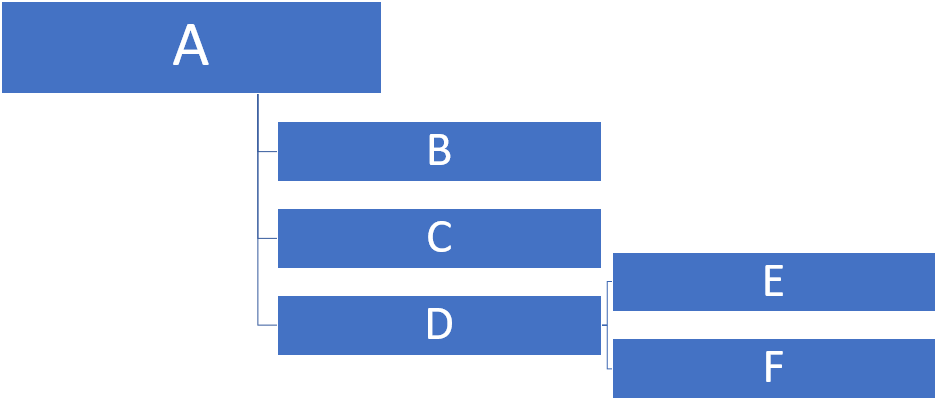
\includegraphics[width=10cm]{img/reddit_utterance_construction.PNG}
	\caption{Exemplary tree how the comment tree is structured for a single thread. A stands for the threads root node and B to F are comments.}
	\label{fig:data:reddit:utterance:construction}
\end{figure}

\section{Vocabulary and Coverage}
\label{data:word_coverage}
After the datasets for both corpora have been generated, we go on with generating corpus specific vocabularies. We do this by iterating the generated dataset and extracting all words that occur there. These collected words are then ranked by their frequency of occurence and converted into vocabularies containing the $n$ most used words, where $n$ stands for the number of words chosen. We decided that we would use three different vocabulary sizes: $25'000$, $50'000$ and $100'000$. As expected, the larger the vocabularies get, the better the coverage is (see Table~\ref{tbl:data:split:corpus:analyze}).
\\
\begin{table}[H]
	\begin{adjustbox}{max width=\textwidth}
		\centering
		\begin{tabular}{lcccccc}
			\toprule
			&\specialcell{Size\\ {[Thousand]}}
			&\specialcell{No. of Words\\ {[Thousand]}}
			&\specialcell{No. of known Words\\ {[Thousand]}}
			&\specialcell{Perc. of known Words \\ {[\%]}}
			&\specialcell{No. of unknown Words \\ {[Thousand]}}
			&\specialcell{Perc. of unknown Words \\ {[\%]}}\\
			\midrule
			OpenSubtitles	&$25$		&$2362$	&$2096$	&$88.73\%$ &$266$	&$11.27\%$\\
							&$50$		&$2362$	&$2116$	&$89.57\%$	&$246$	&$10.43\%$\\
							&$100$	&$2362$	&$2127$	&$90.03\%$	&$236$	&$9.97\%$\\\\
			Reddit		&$25$		&$1717$	&$1683$	&$98.00\%$	&$34$		&$2.00\%$\\
						&$50$		&$1717$	&$1699$	&$98.98\%$	&$17$		&$1.02\%$\\
						&$100$	&$1717$	&$1707$	&$99.42\%$	&$10$		&$0.58\%$\\
			\bottomrule
		\end{tabular}
	\end{adjustbox}
	\caption{Word coverage of differently sized vocabularies extracted from the generated datasets.}
	\label{tbl:data:split:corpus:analyze}
\end{table}

Figure~\ref{fig:data:reddit:vocab:analyze} shows what percentage of the words in an utterance is missing using the specified vocabulary. It shows that the coverage of the Reddit vocabularies is much bigger than the OpenSubtitles.\todo{Begründung? es befinden sich viele Sätze mehrfach im Datensatz.}

\begin{figure}[H]
	\minipage{0.5\textwidth}
	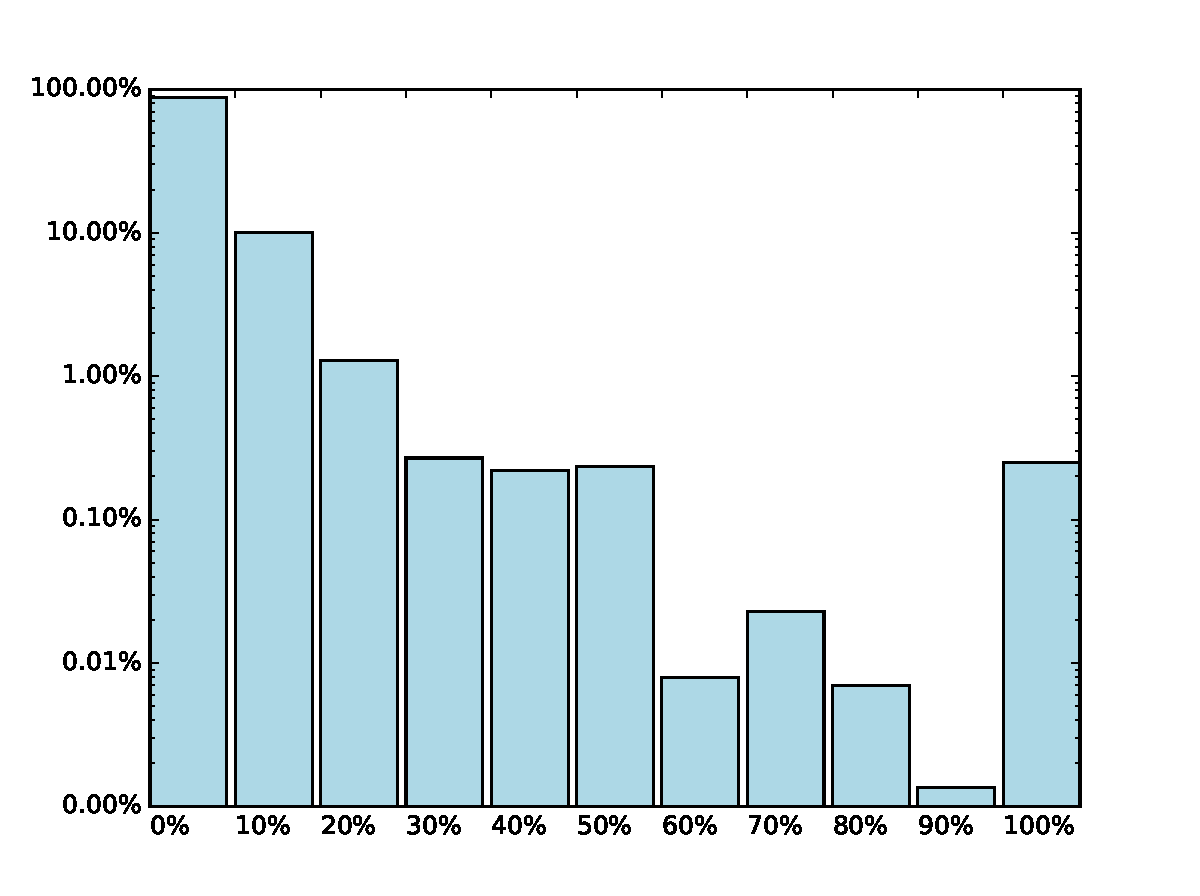
\includegraphics[width=\linewidth]{img/reddit_vocab_analyze_100k_perc.pdf}
	\centering
	\small
	\text{Reddit 100k}
	\endminipage\hfill
	\minipage{0.5\textwidth}
	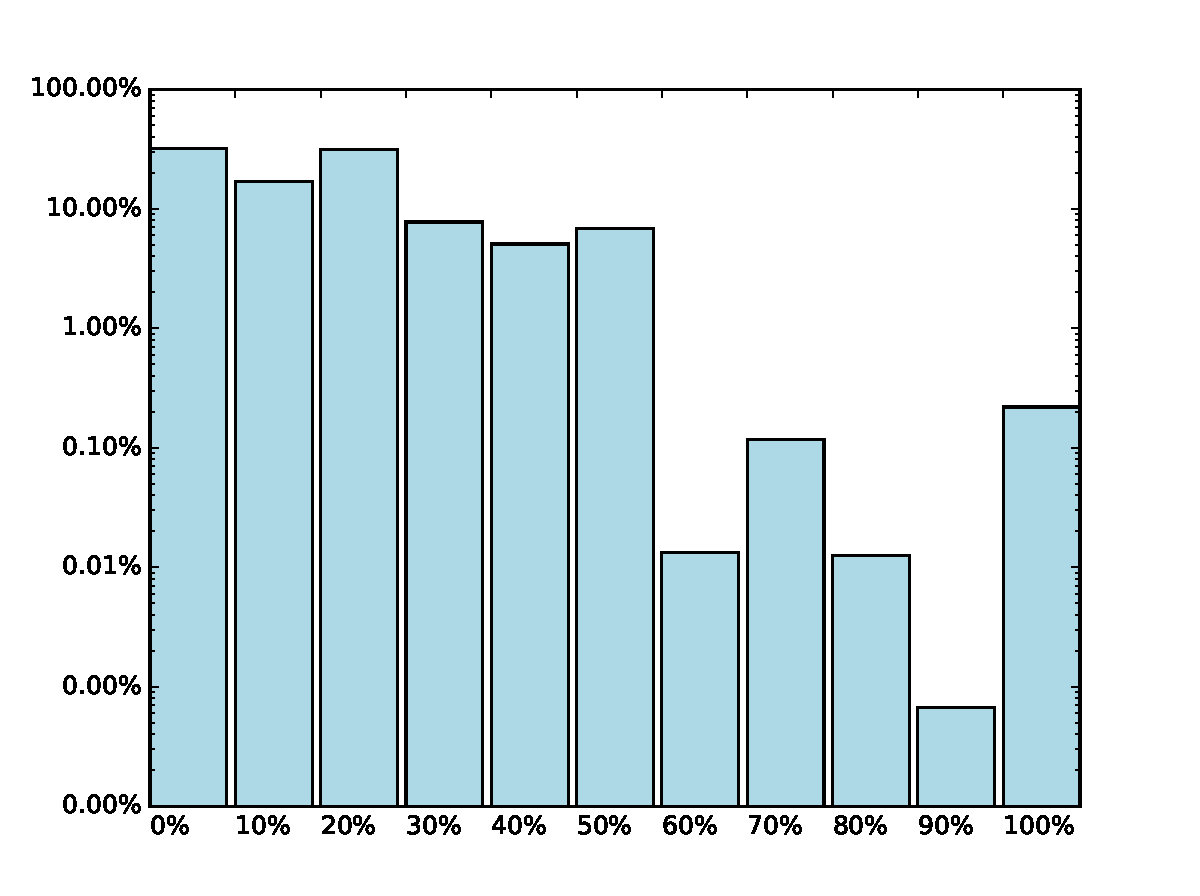
\includegraphics[width=\linewidth]{img/opus_vocab_analyze_100k_perc.pdf}
	\centering
	\small
	\text{OpenSubtitles 100k}
	\endminipage\hfill
	\minipage{0.5\textwidth}
	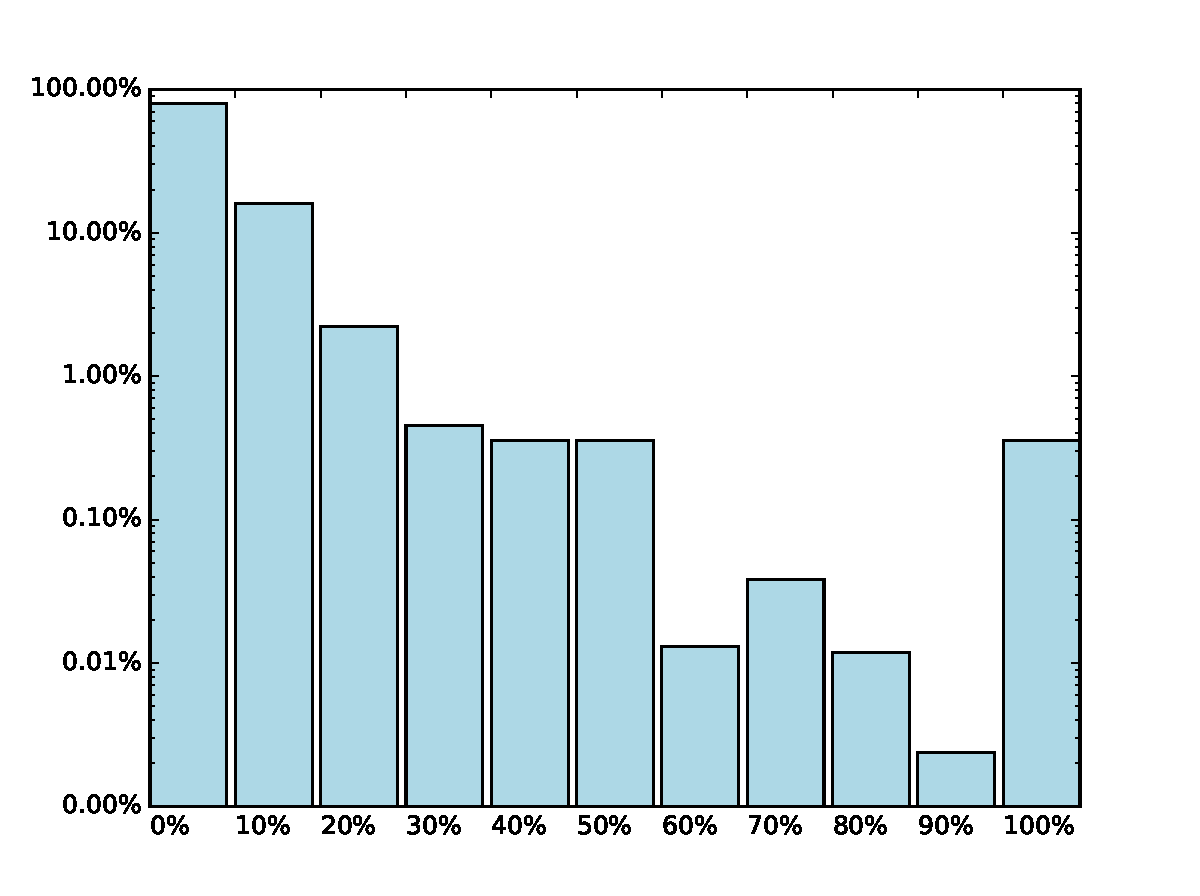
\includegraphics[width=\linewidth]{img/reddit_vocab_analyze_50k_perc.pdf}
	\centering
	\small
	\text{Reddit 50k}
	\endminipage\hfill
	\minipage{0.5\textwidth}
	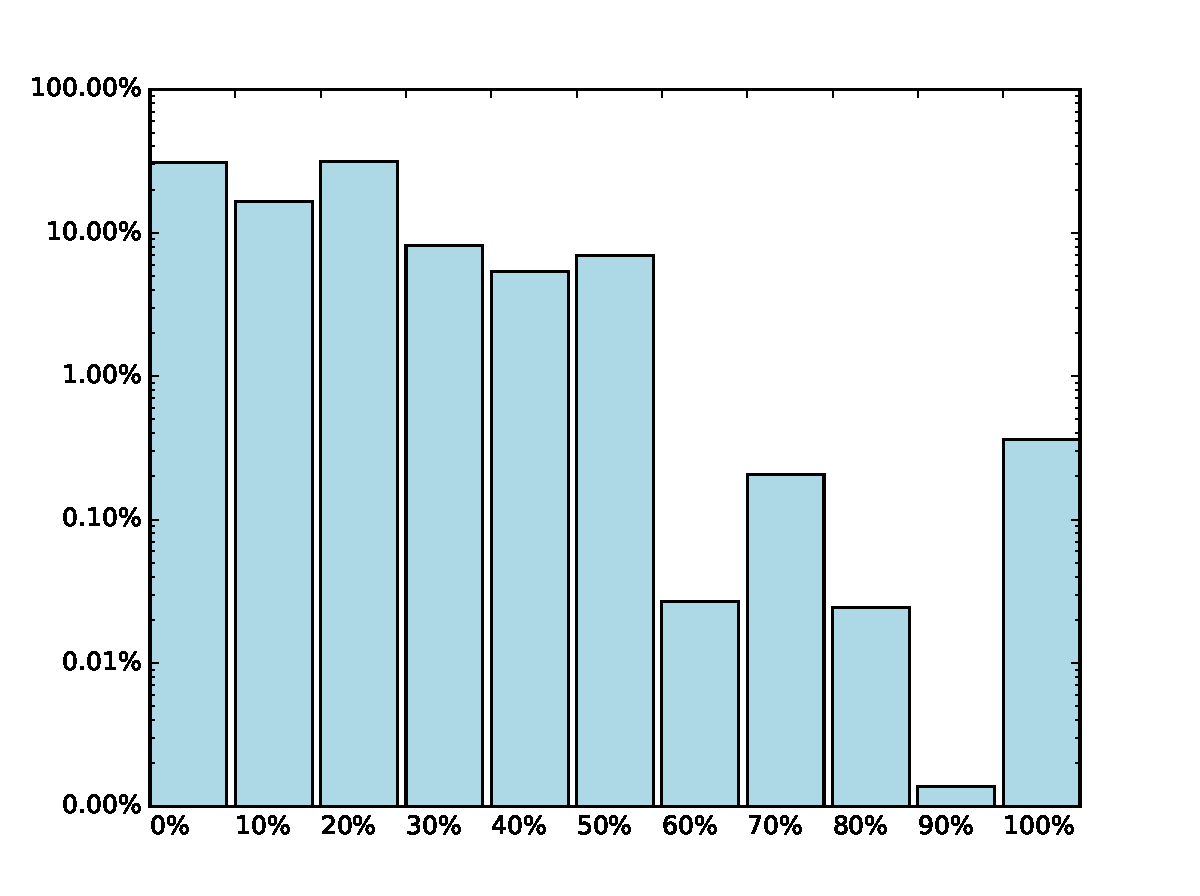
\includegraphics[width=\linewidth]{img/opus_vocab_analyze_50k_perc.pdf}
	\centering
	\small
	\text{OpenSubtitles 50k}
	\endminipage\hfill
	\minipage{0.5\textwidth}%
	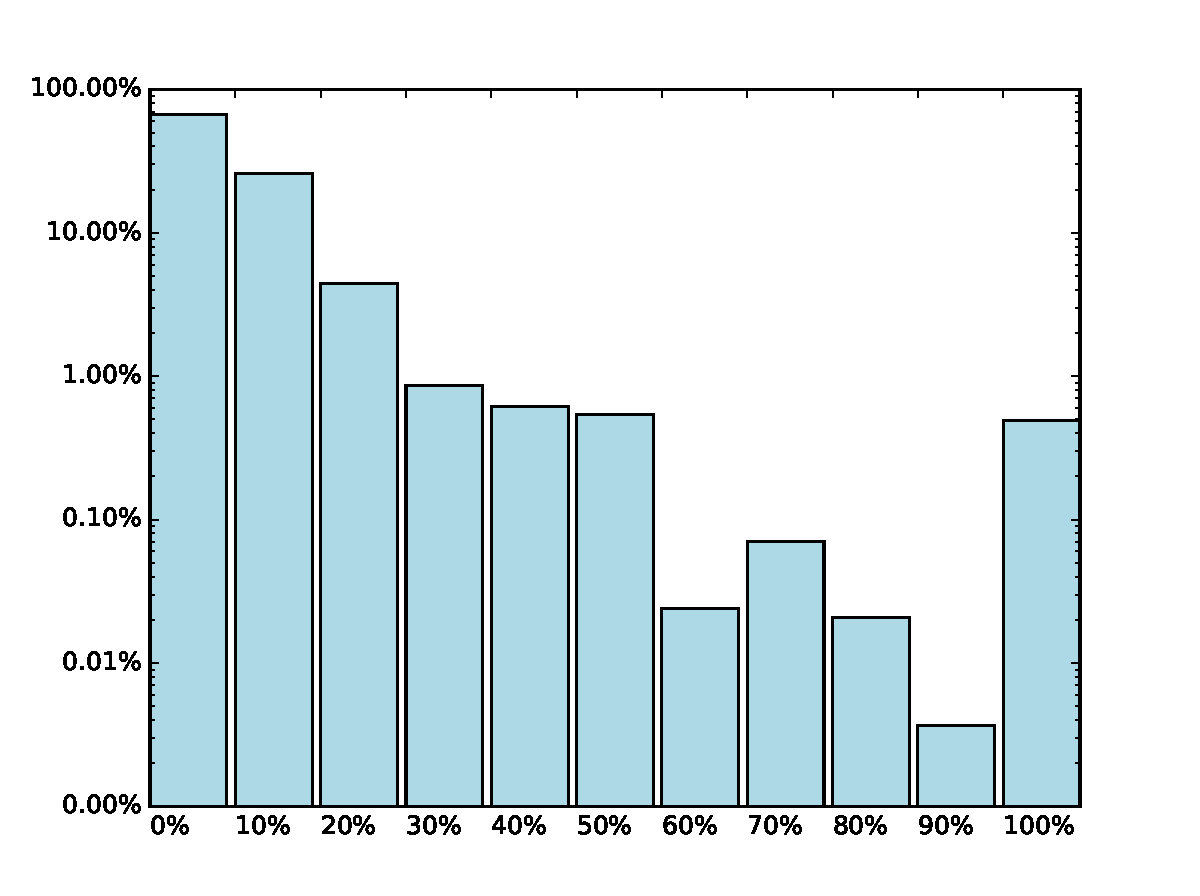
\includegraphics[width=\linewidth]{img/reddit_vocab_analyze_25k_perc.pdf}
	\centering
	\small
	\text{Reddit 25k}
	\endminipage\hfill
	\minipage{0.5\textwidth}%
	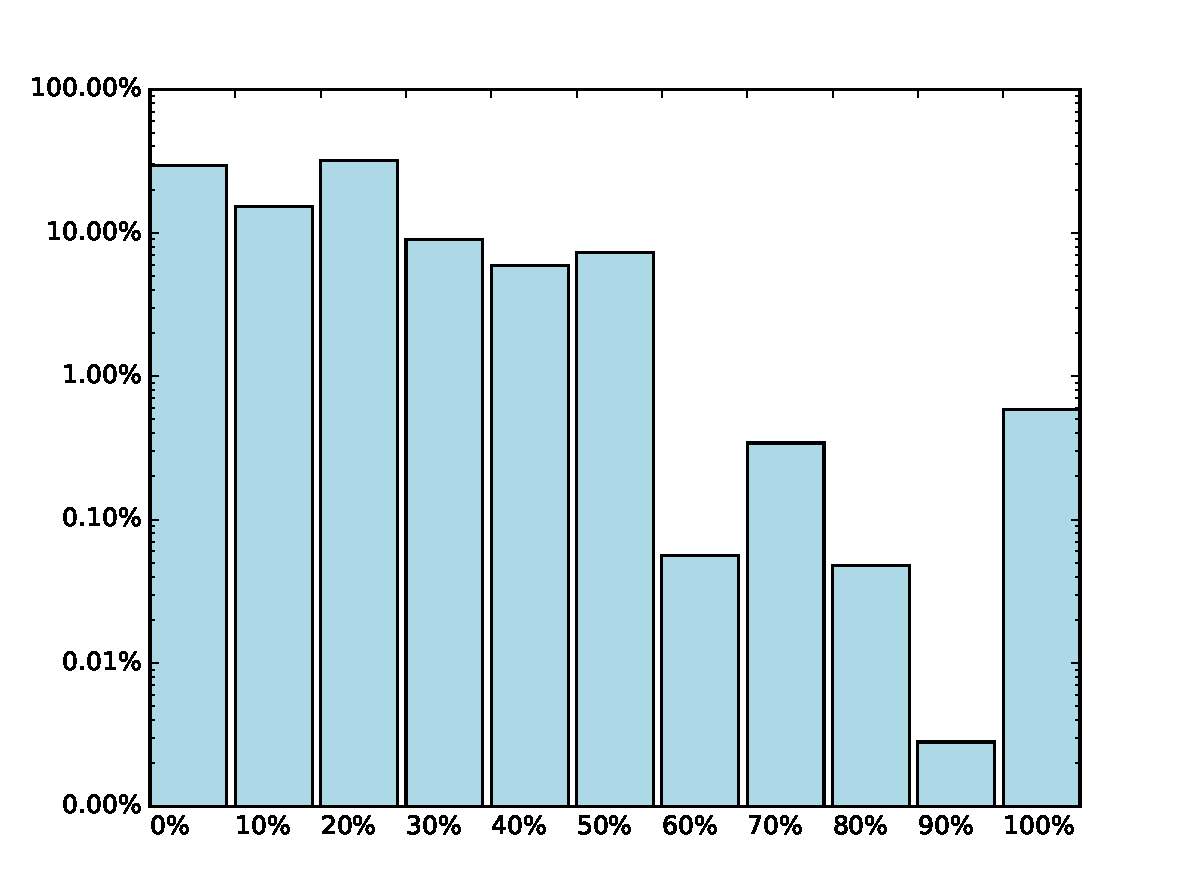
\includegraphics[width=\linewidth]{img/opus_vocab_analyze_25k_perc.pdf}
	\centering
	\small
	\text{OpenSubtitles 25k}
	\endminipage
	\caption{Plots (y-logarithmic) showing the percentage of words missing per utterance for specific vocabulary sizes.}
	\label{fig:data:reddit:vocab:analyze}
\end{figure}
\todo{Wollen wir darauf eingehen, weshalb log plot?}

\section{Splitting the Datasets}
\label{data:split_corpus}
The generated datasets have to be split in order to obtain a train, validation, and test datasets. The table \ref{tbl:data:split:corpus} shows how proportions in which the datasets were split. We split in a way, that we always process two utterances at one to ensure that there is no overlap between the training and the other datasets. The splitting is also done randomly, to ensure that we do not run into problems due to the fact that the utterances may be sorted in any unknown way.
\\
\begin{table}[H]
	\centering
	\begin{adjustbox}{max width=\textwidth}
		\centering
		\begin{tabular}{llccc}
			\toprule
			&  \specialcell{Set}
			&  \specialcell{Share of Dataset \\ {[\%]}}
			&  \specialcell{Size \\{[MB]}}
			&  \specialcell{No. of Lines \\{[Thousand]}}\\
			\midrule
			OpenSubtitles	& Train	&97\%	&9'393	&321'643	\\
			&Valid	&1\%	&97		&3'315	\\
			&Test	&2\%	&194	&6'631	\\
			\midrule
			Reddit			&Train	&97\%	&8'455	&75'297	\\
			&Valid	&2\%	&185	&1'552	\\
			&Test	&1\%	&92		&776	\\
			\bottomrule
		\end{tabular}
	\end{adjustbox}
	\caption{Proportion in which the datasets were split to obtain a train, validation and test set.}
	\label{tbl:data:split:corpus}
\end{table}

\section{Time-Lag Analysis OpenSubtitles}
\label{data:opensubtitles:time_lag_analysis}
While searching through the OpenSubtitles dataset, we discovered that there are several pairs of utterances which don't make a lot of sense (e.g. (``I love cupcake'', ``Hello, how are you?'')) under the viewpoint of conversational modeling. We quickly realized that this useless pairs of utterances occur because of the way we preprocess the raw corpus: In order to get a sample, we take the first utterance and combine it with the utterance on the next line in the preprocessed corpus. The problem occurs when the timestamps signify a large time difference between the first and second utterance. This is understandable, as all utterances are just saved in the corpus one after the other without taking timestamps (see OpenSubtitles paragraph in Chapter~\ref{data:structure_of_corpora}) into account. In order to investigate if this problem is urgent, we did an analysis to see if what proportion of utterances have a time-lag higher than a certain timespan. The results of this investigation are summarized in Figure~\ref{fig:data:analyse:timediff:opus}.

\begin{figure}[H]
	\centering
	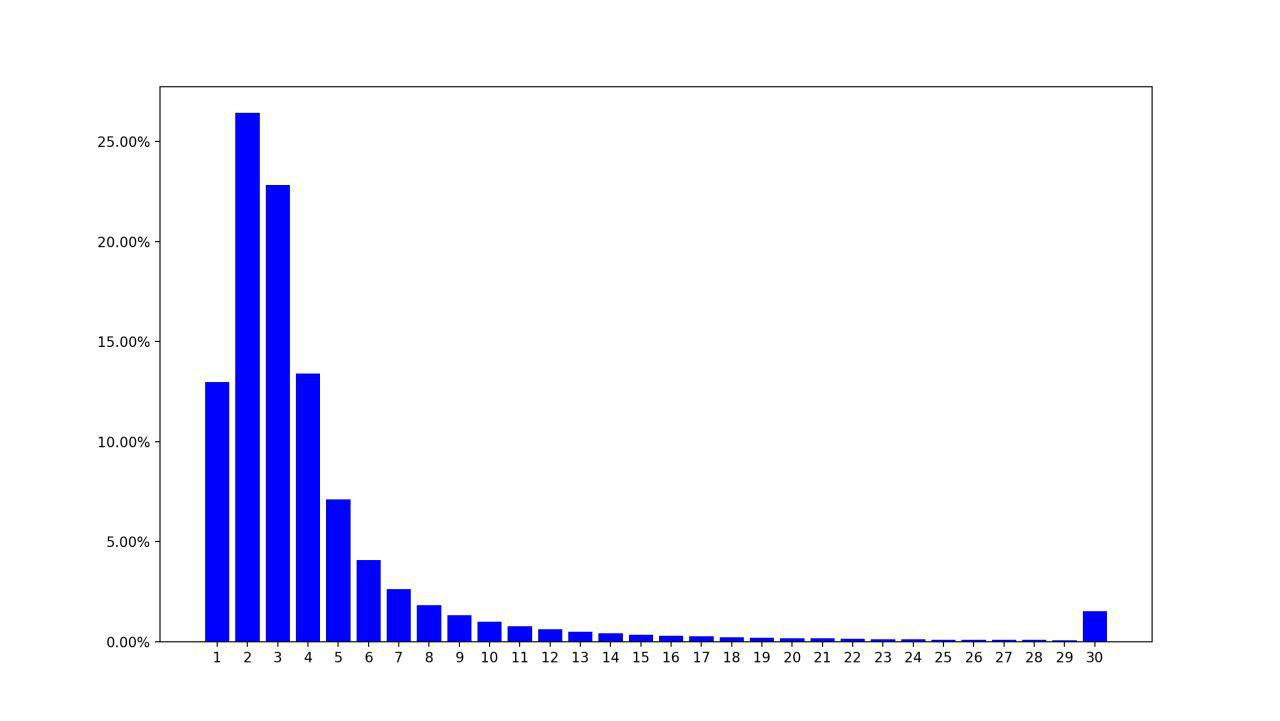
\includegraphics[width=15cm]{img/opus_time_analyze.PNG}
	\caption{Relative distribution (discrete) of the time-lag between two utterances in the raw OpenSubtitles corpus. Most of the utterances lie in the range from $1$ to $5$ seconds: $13.0\%$ within 1 second, $26.4\%$ within 2 seconds, $22.8\%$ within 3 seconds, $13.4\%$ within 4 seconds and  $7.0\%$ within 5 seconds.}
	\label{fig:data:analyse:timediff:opus}
\end{figure}

As one can see, over 80\% of the utterances occur within one to five seconds of one another. The spike at the end of the graph occurs because there might be changes in the scenes of the movies, which can lead to two consecutive utterances in the corpus being uttered after a larger gap. The other reason is, that each movie is stored in a single file and hence, there might be utterances which are combined, but actually belong to two different movies.

As this analysis has shown, most utterances lie so close to one another that this will most probably not be a problem when training our model with them.

\section{N-Gram Analysis}
\label{chapter:data:ngram}
We also do an n-gram analysis of the used corpora. For this purpose, we generated uni- and bigrams for both the OpenSubtitles and Reddit corpora. We do this so that we can compare the n-grams of the outputs produced by our models after they have been trained with the n-grams obtained when analyzing the preprocessed corpora. This enables us to find correlations between the n-grams produced by this analysis and n-grams extracted from the outputs of the trained models. The results of analyzing the preprocessed datasets are visualized in the figures~\ref{data:ngram:freq_top_30} and \ref{data:ngram:graph_top_50}. For the second visualizations, we use a custom graph visualization which we call ``N-Gram Graph''. This allows us to visualize how n-grams can be connected to each other (through edges) and at the same time visualize their relative occurrence frequencies to all other n-grams in the graph.\todo{What to do with the graphs?!}
 
\begin{figure}[H]
	\minipage{0.5\textwidth}
	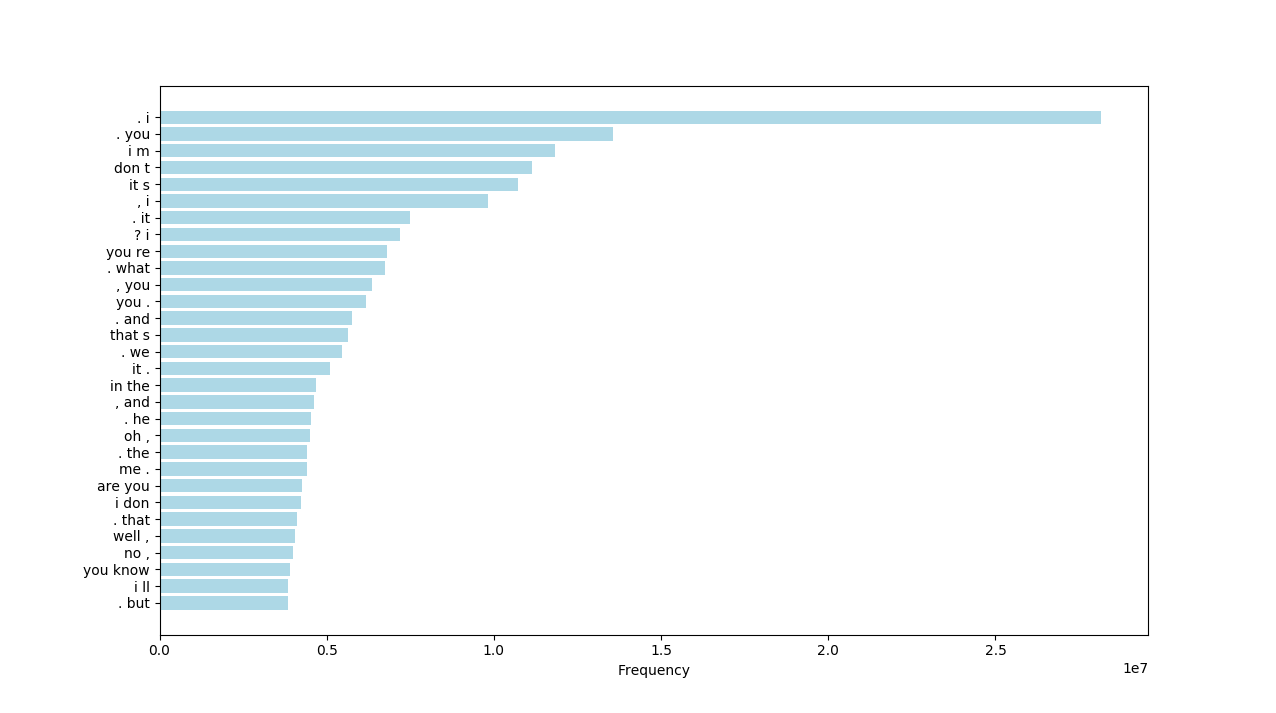
\includegraphics[width=\linewidth]{img/opensubtitles_bigram_top_30_freq}
	\centering
	\small
	\text{OpenSubtitles}
	\endminipage\hfill
	\minipage{0.5\textwidth}
	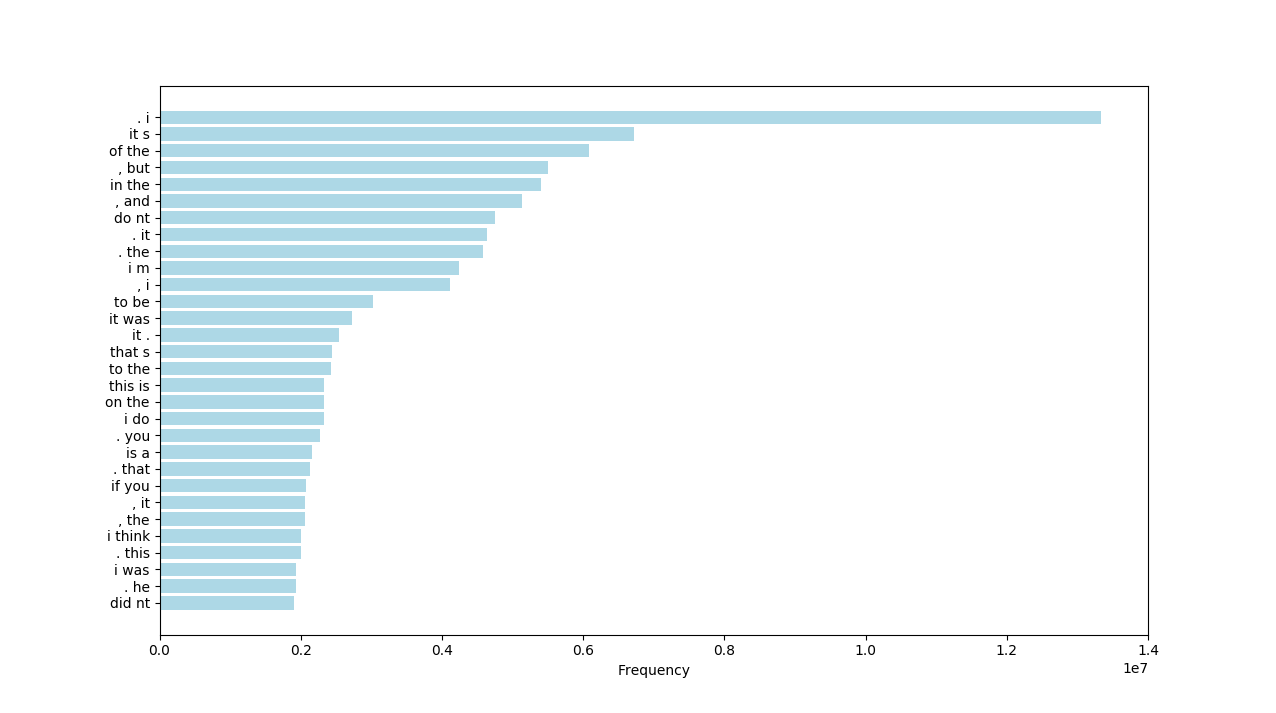
\includegraphics[width=\linewidth]{img/reddit_bigram_top_30_freq}
	\centering
	\small
	\text{Reddit}
	\endminipage\hfill
	\caption{Occurrence frequencies of the 30 most used bigrams in the OpenSubtitles~(left) and Reddit (right) datasets.}
	\label{data:ngram:freq_top_30}
\end{figure}

\begin{figure}[H]
	\minipage{1\textwidth}
	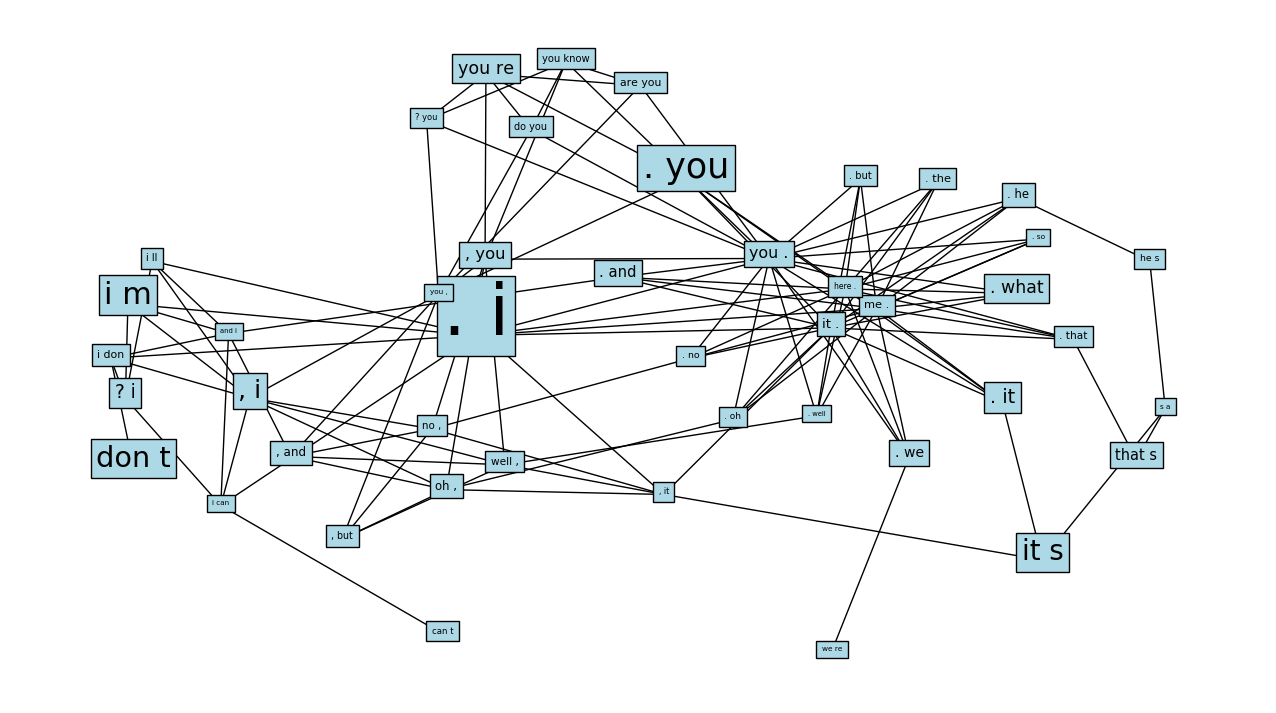
\includegraphics[width=\linewidth]{img/opensubtitles_bigram_top_50_graph}
	\centering
	\small
	\text{OpenSubtitles}
	\endminipage\hfill
	\minipage{1\textwidth}
	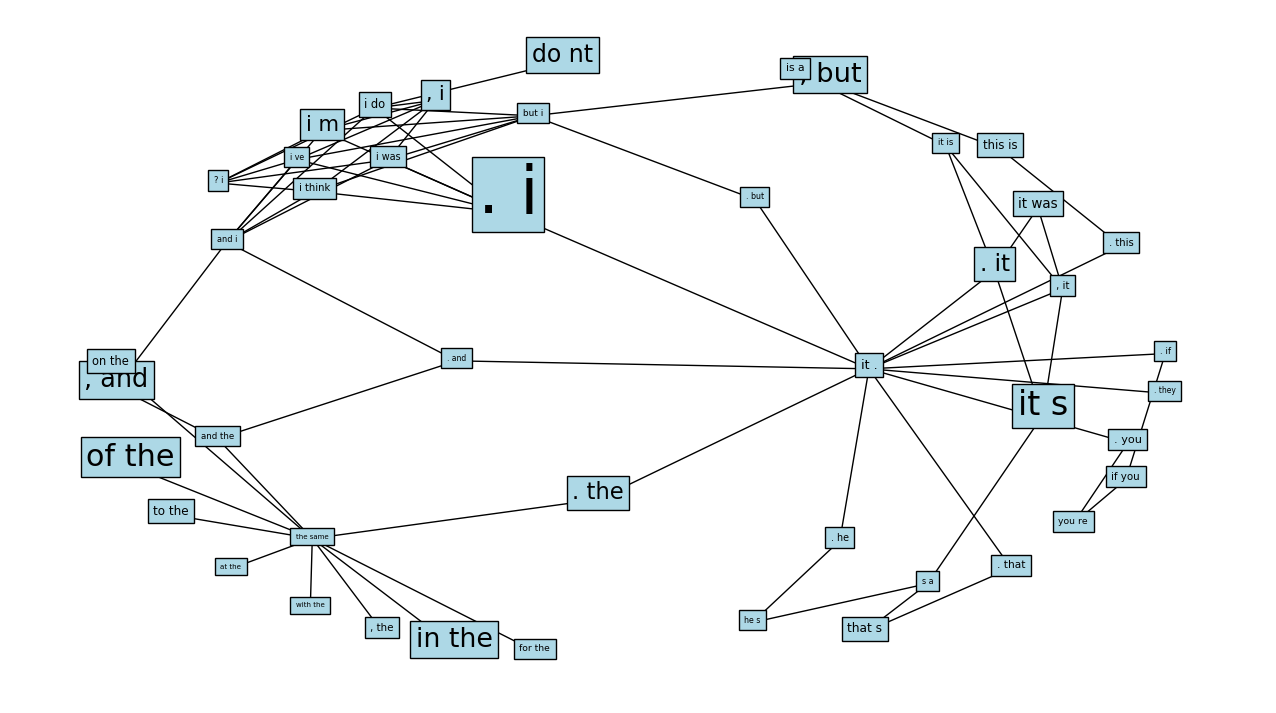
\includegraphics[width=\linewidth]{img/reddit_bigram_top_50_graph}
	\centering
	\small
	\text{Reddit}
	\endminipage\hfill
	\caption{N-Gram graphs for the 50 most used bigrams in the OpenSubtitles (upper) and Reddit (lower) datasets. Each node in the graphs represents a bigram, the edges between them show that either the first word of the first bigram matches the second word of the other bigram or the last word of the first bigram equals the last word of the second bigram. The size of each node is relative to its occurrence frequency, which means, that larger nodes occur more frequent than smaller ones.}
	\label{data:ngram:graph_top_50}
\end{figure}

